\section{Sample System Ouput - Raw Data}
\begin{figure}[H]
	\centering
	\caption{accelX vs. Time}
		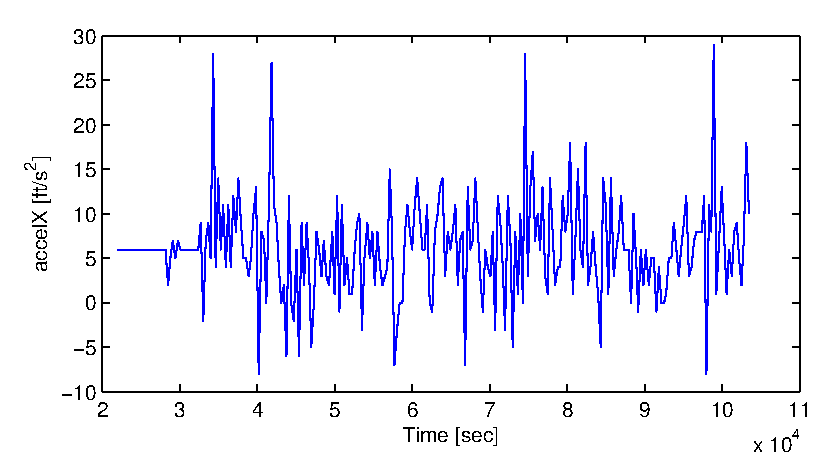
\includegraphics[width = 0.7\textwidth]{C:/Users/mufasa/Documents/Thesis/LaTex/figures/sampleOutput/Raw/accelX.eps}
\end{figure}
\begin{figure}[H]
	\centering
	\caption{accelY vs. Time}
		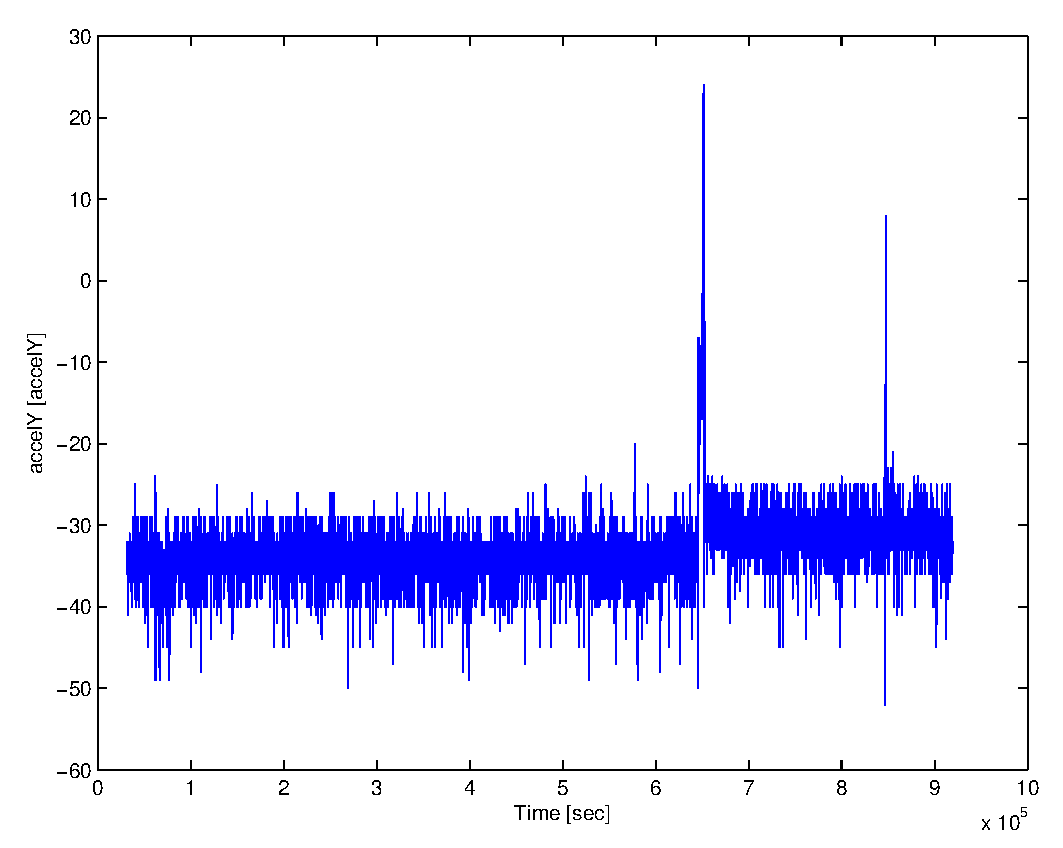
\includegraphics[width = 0.7\textwidth]{C:/Users/mufasa/Documents/Thesis/LaTex/figures/sampleOutput/Raw/accelY.eps}
\end{figure}
\begin{figure}[H]
	\centering
	\caption{accelZ vs. Time}
		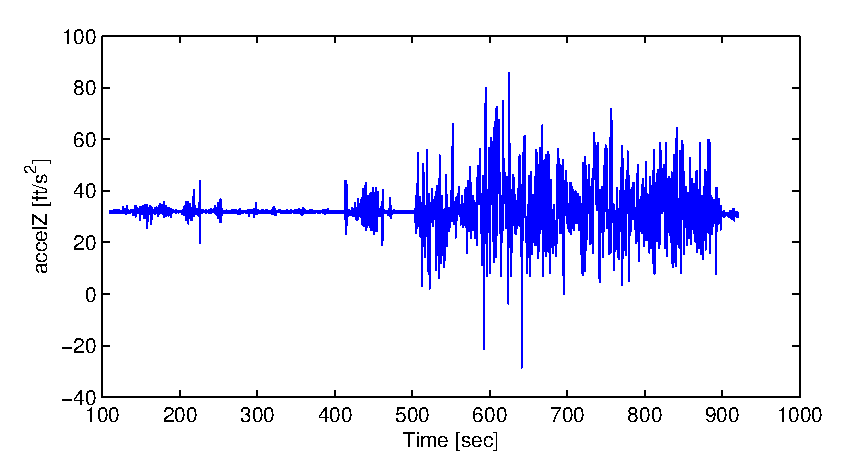
\includegraphics[width = 0.7\textwidth]{C:/Users/mufasa/Documents/Thesis/LaTex/figures/sampleOutput/Raw/accelZ.eps}
\end{figure}
\begin{figure}[H]
	\centering
	\caption{gyroX vs. Time}
		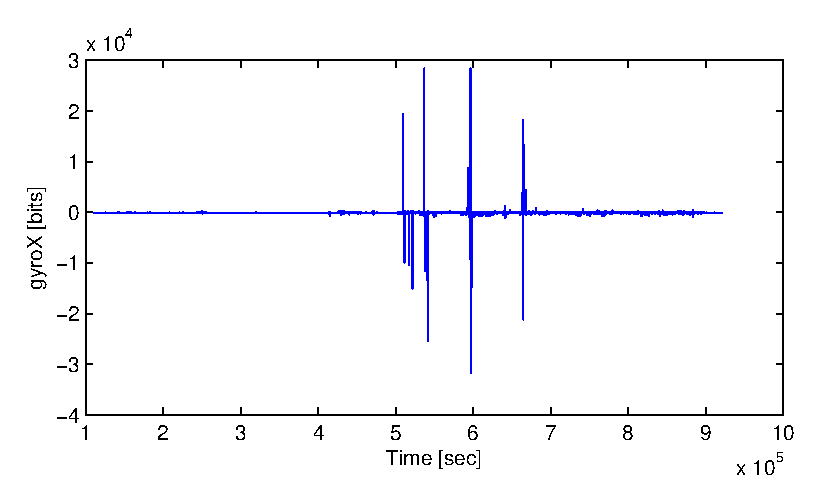
\includegraphics[width = 0.7\textwidth]{C:/Users/mufasa/Documents/Thesis/LaTex/figures/sampleOutput/Raw/gyroX.eps}
\end{figure}
\begin{figure}[H]
	\centering
	\caption{gyroY vs. Time}
		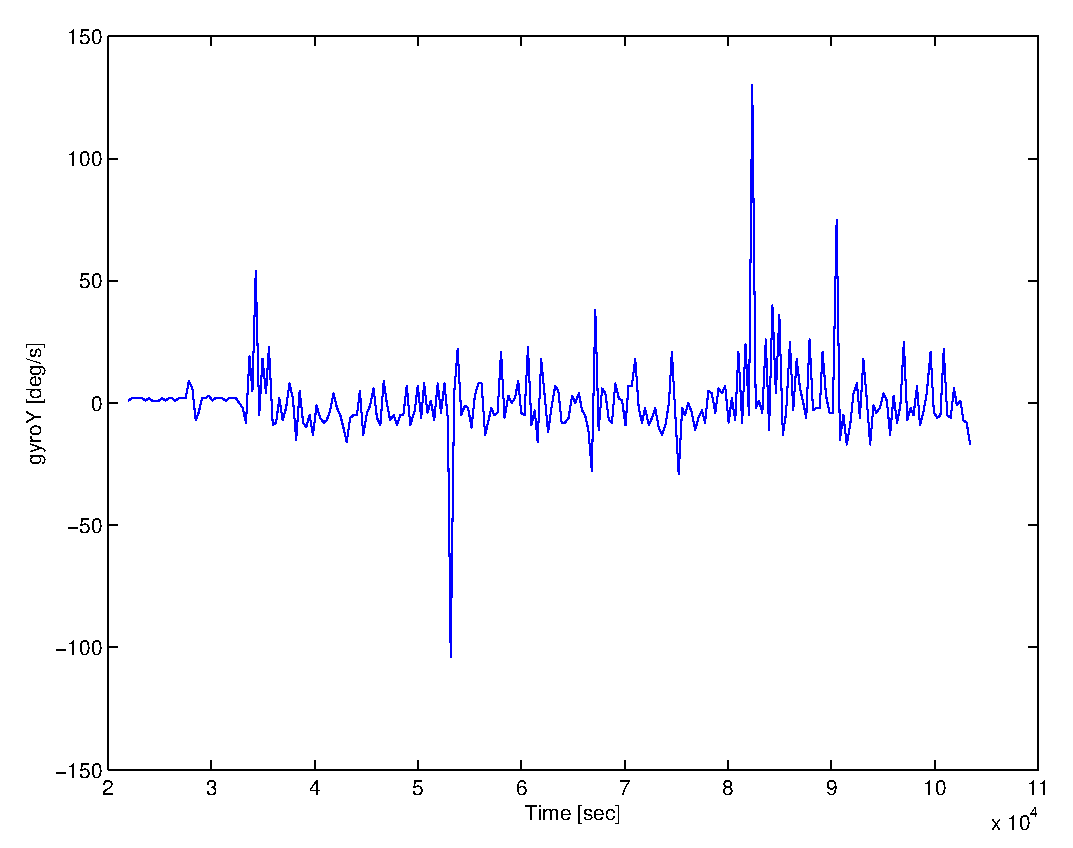
\includegraphics[width = 0.7\textwidth]{C:/Users/mufasa/Documents/Thesis/LaTex/figures/sampleOutput/Raw/gyroY.eps}
\end{figure}
\begin{figure}[H]
	\centering
	\caption{gyroZ vs. Time}
		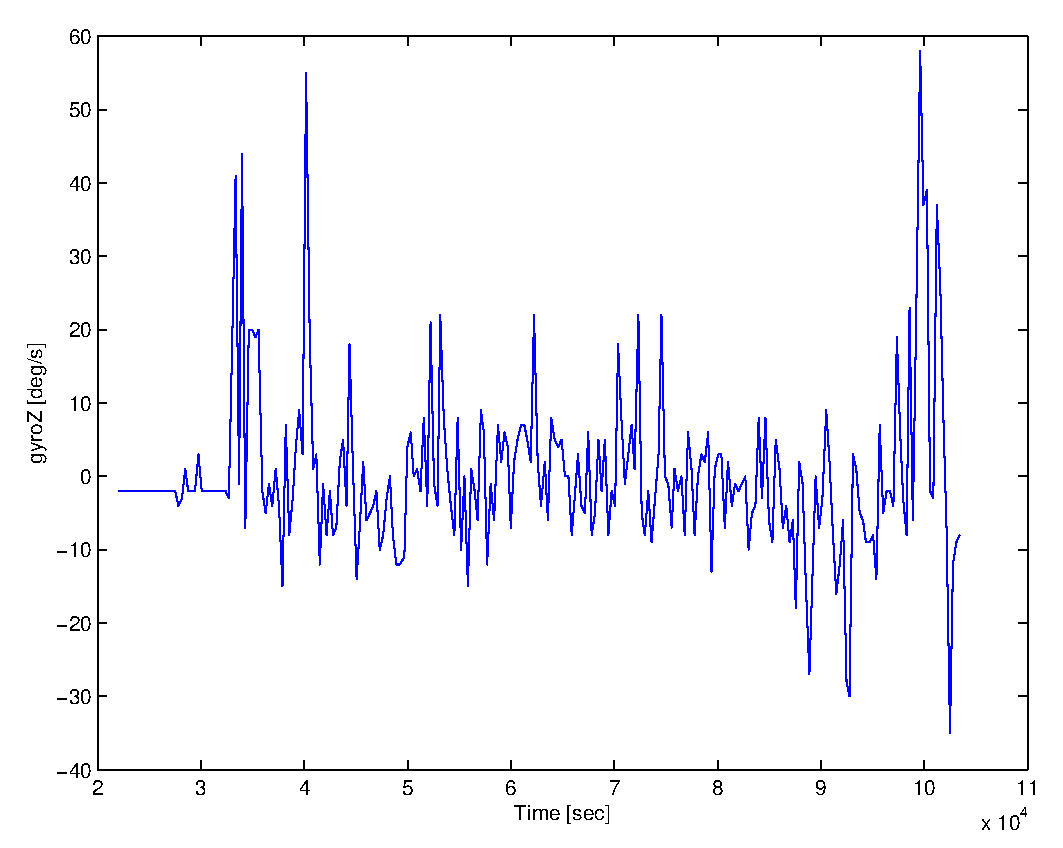
\includegraphics[width = 0.7\textwidth]{C:/Users/mufasa/Documents/Thesis/LaTex/figures/sampleOutput/Raw/gyroZ.eps}
\end{figure}
\begin{figure}[H]
	\centering
	\caption{magX vs. Time}
		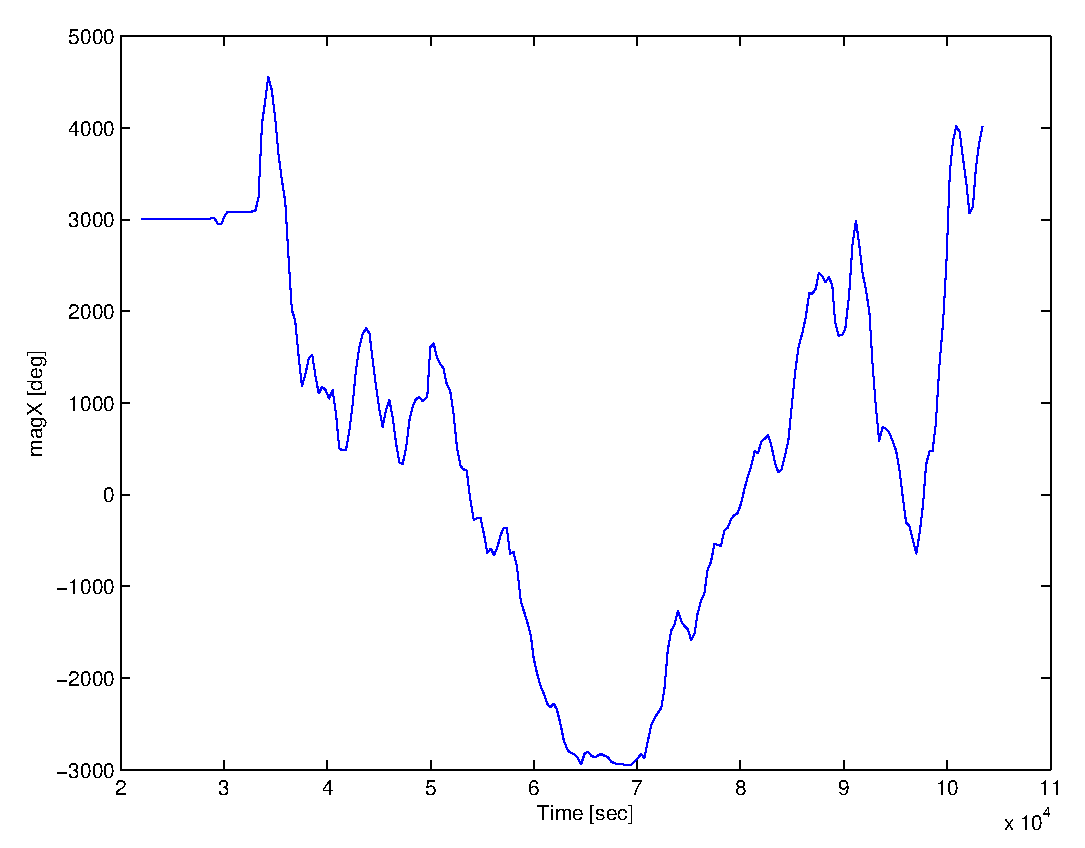
\includegraphics[width = 0.7\textwidth]{C:/Users/mufasa/Documents/Thesis/LaTex/figures/sampleOutput/Raw/magX.eps}
\end{figure}
\clearpage
\begin{figure}[H]
	\centering
	\caption{magY vs. Time}
		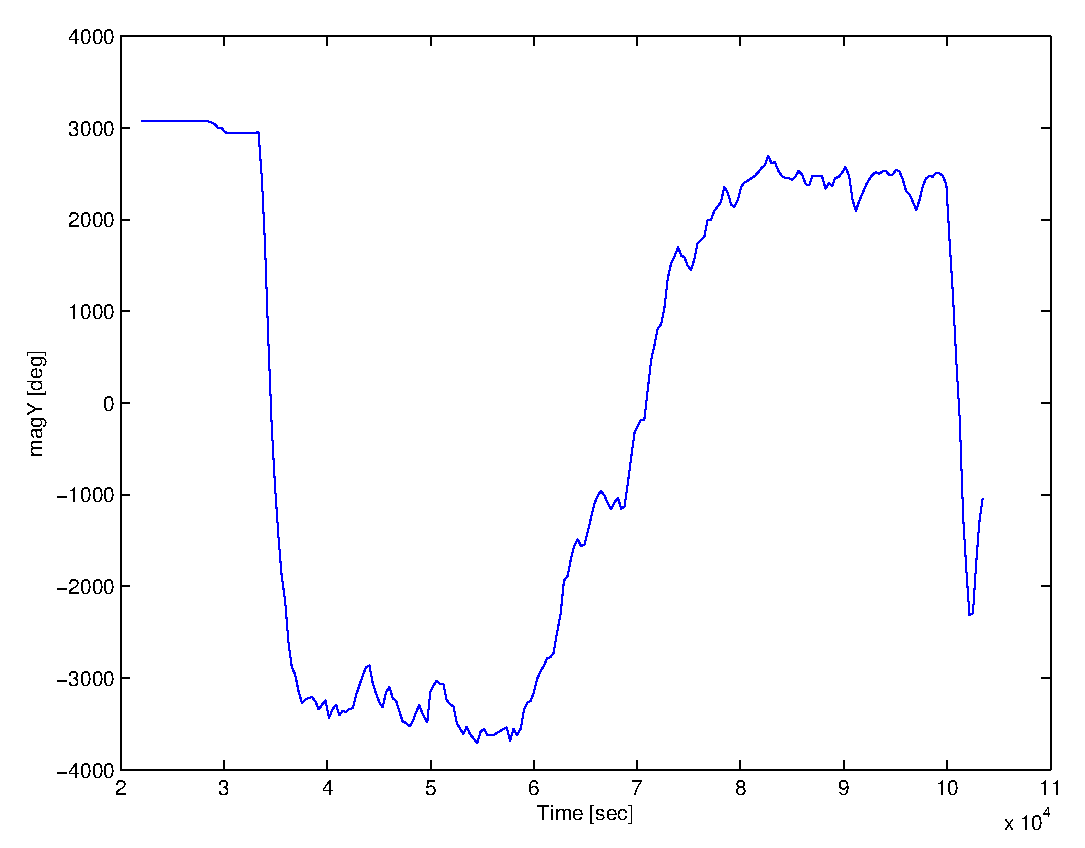
\includegraphics[width = 0.7\textwidth]{C:/Users/mufasa/Documents/Thesis/LaTex/figures/sampleOutput/Raw/magY.eps}
\end{figure}
\begin{figure}[H]
	\centering
	\caption{magZ vs. Time}
		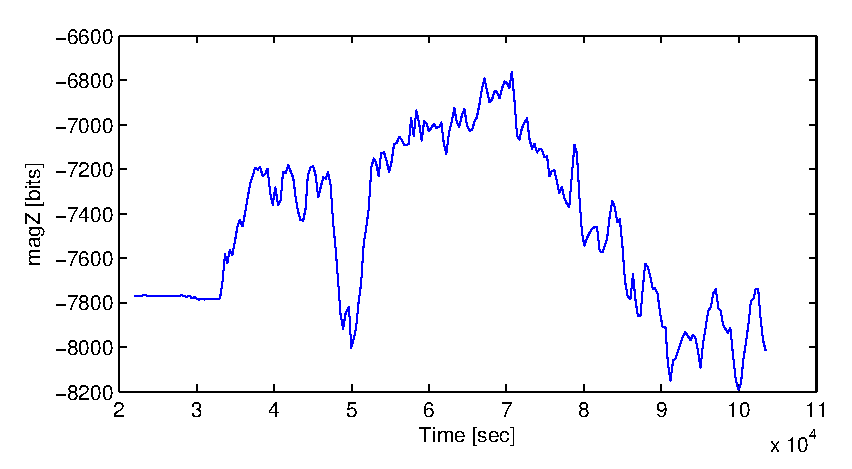
\includegraphics[width = 0.7\textwidth]{C:/Users/mufasa/Documents/Thesis/LaTex/figures/sampleOutput/Raw/magZ.eps}
\end{figure}
\begin{figure}[H]
	\centering
	\caption{hmcX vs. Time}
		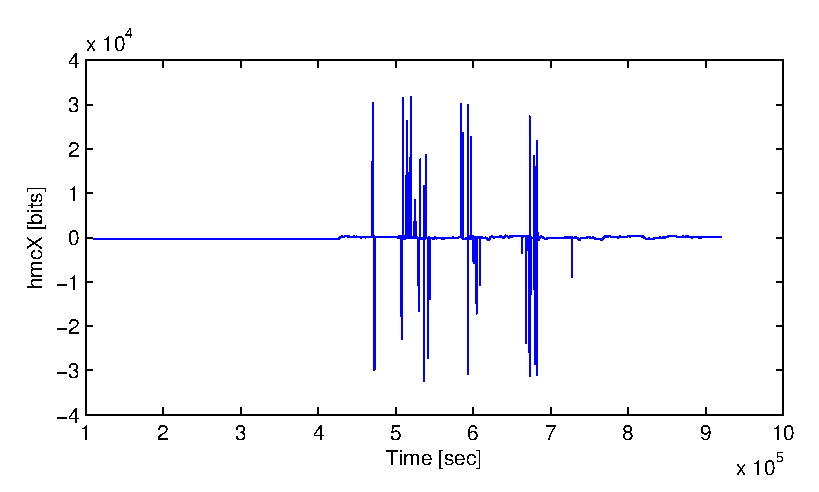
\includegraphics[width = 0.7\textwidth]{C:/Users/mufasa/Documents/Thesis/LaTex/figures/sampleOutput/Raw/hmcX.eps}
\end{figure}
\begin{figure}[H]
	\centering
	\caption{hmcZ vs. Time}
		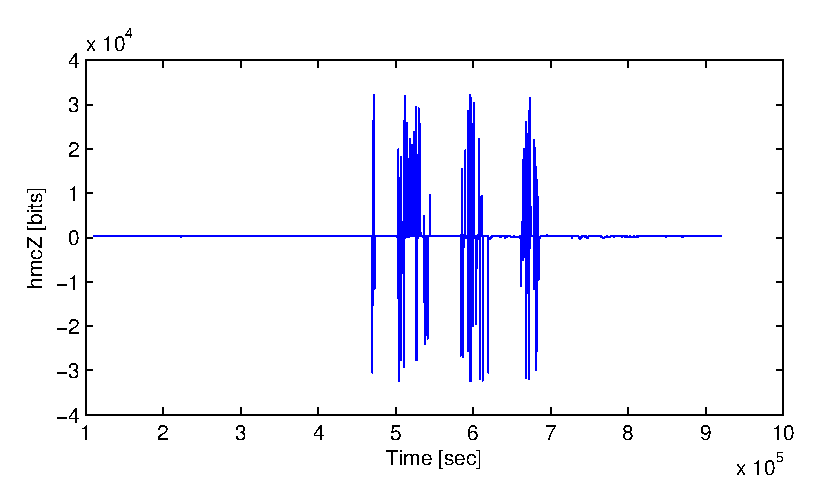
\includegraphics[width = 0.7\textwidth]{C:/Users/mufasa/Documents/Thesis/LaTex/figures/sampleOutput/Raw/hmcZ.eps}
\end{figure}
\begin{figure}[H]
	\centering
	\caption{hmcY vs. Time}
		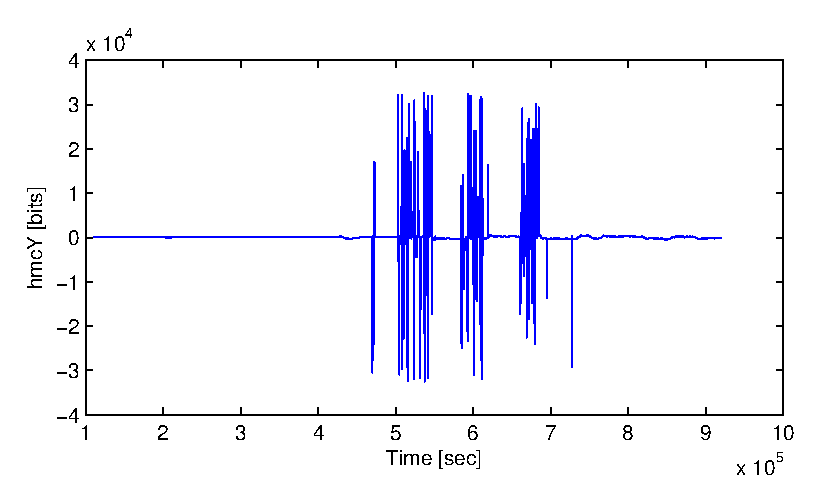
\includegraphics[width = 0.7\textwidth]{C:/Users/mufasa/Documents/Thesis/LaTex/figures/sampleOutput/Raw/hmcY.eps}
\end{figure}
\begin{figure}[H]
	\centering
	\caption{press0 vs. Time}
		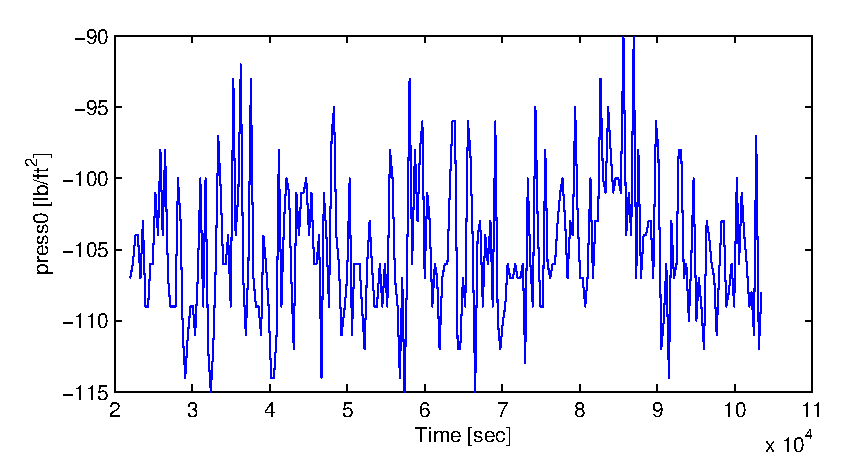
\includegraphics[width = 0.7\textwidth]{C:/Users/mufasa/Documents/Thesis/LaTex/figures/sampleOutput/Raw/press0.eps}
\end{figure}
\begin{figure}[H]
	\centering
	\caption{press1 vs. Time}
		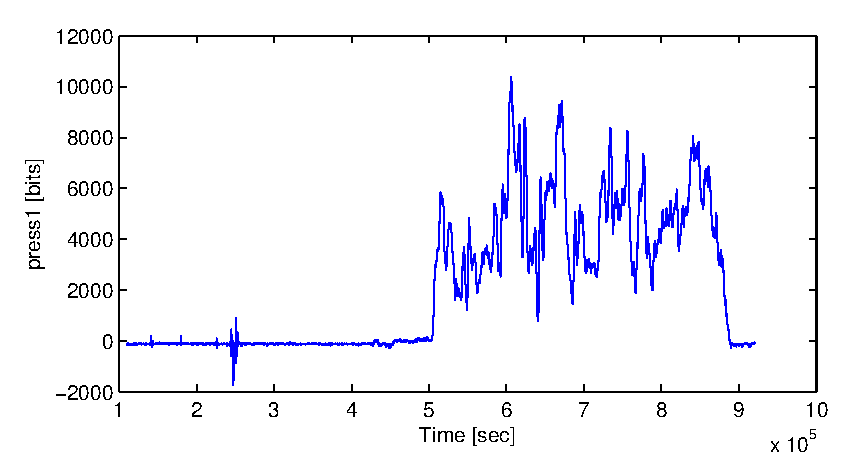
\includegraphics[width = 0.7\textwidth]{C:/Users/mufasa/Documents/Thesis/LaTex/figures/sampleOutput/Raw/press1.eps}
\end{figure}
\begin{figure}[H]
	\centering
	\caption{press2 vs. Time}
		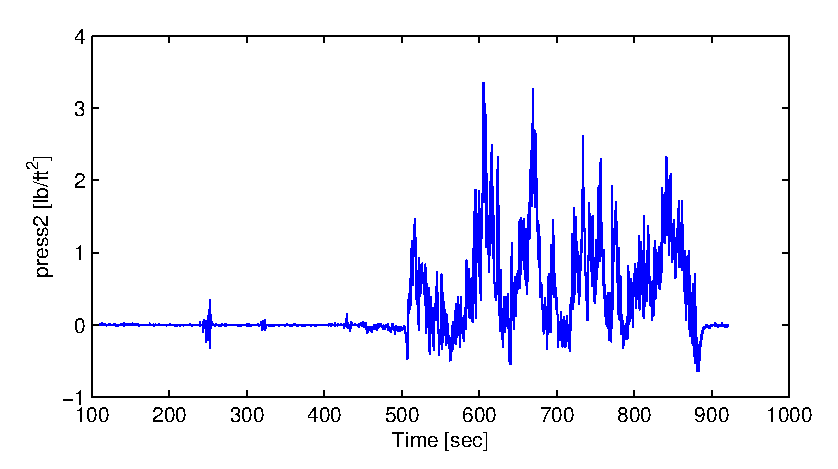
\includegraphics[width = 0.7\textwidth]{C:/Users/mufasa/Documents/Thesis/LaTex/figures/sampleOutput/Raw/press2.eps}
\end{figure}
\begin{figure}[H]
	\centering
	\caption{press3 vs. Time}
		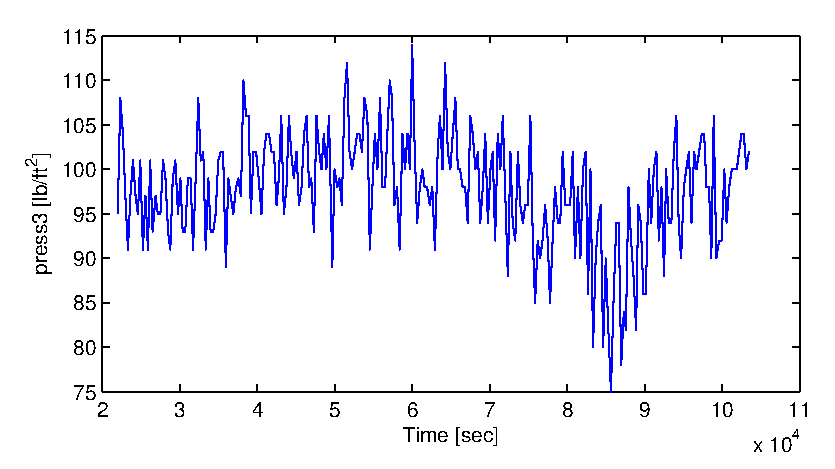
\includegraphics[width = 0.7\textwidth]{C:/Users/mufasa/Documents/Thesis/LaTex/figures/sampleOutput/Raw/press3.eps}
\end{figure}
\begin{figure}[H]
	\centering
	\caption{gpsLat vs. Time}
		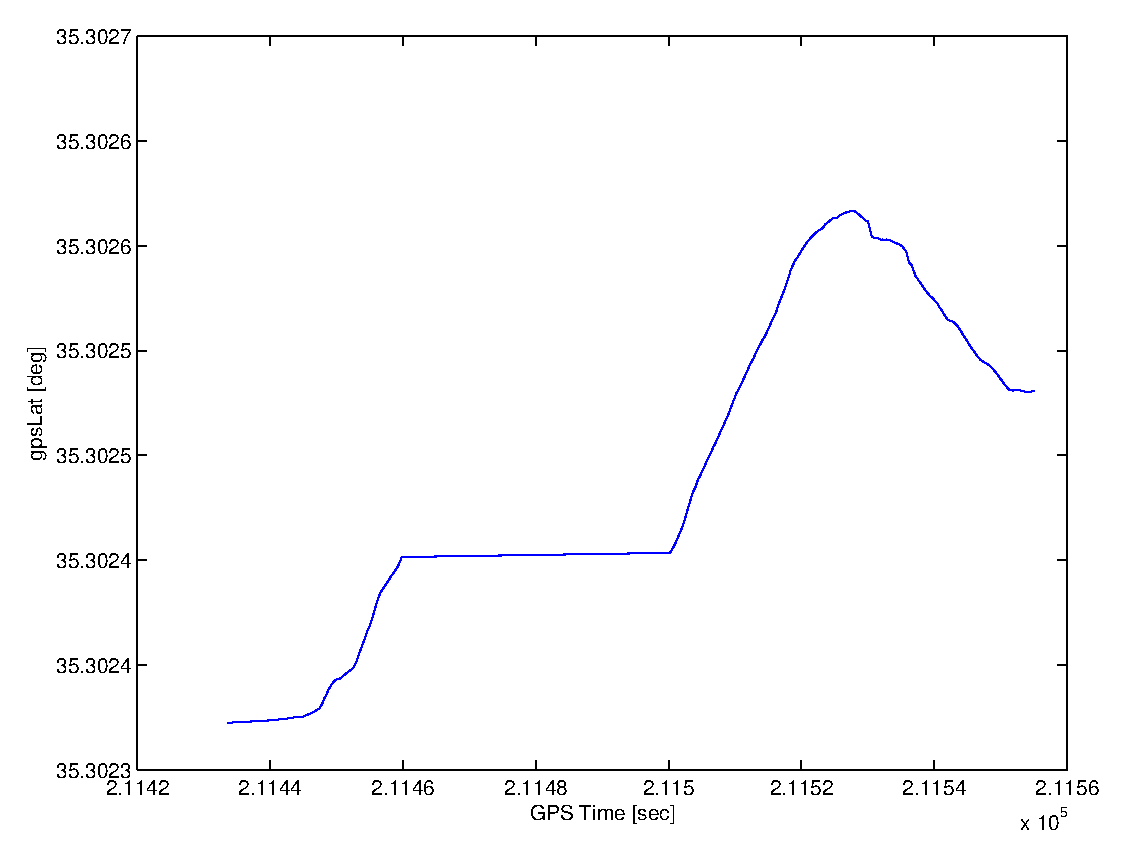
\includegraphics[width = 0.7\textwidth]{C:/Users/mufasa/Documents/Thesis/LaTex/figures/sampleOutput/Raw/gpsLat.eps}
\end{figure}
\begin{figure}[H]
	\centering
	\caption{gpsLong vs. Time}
		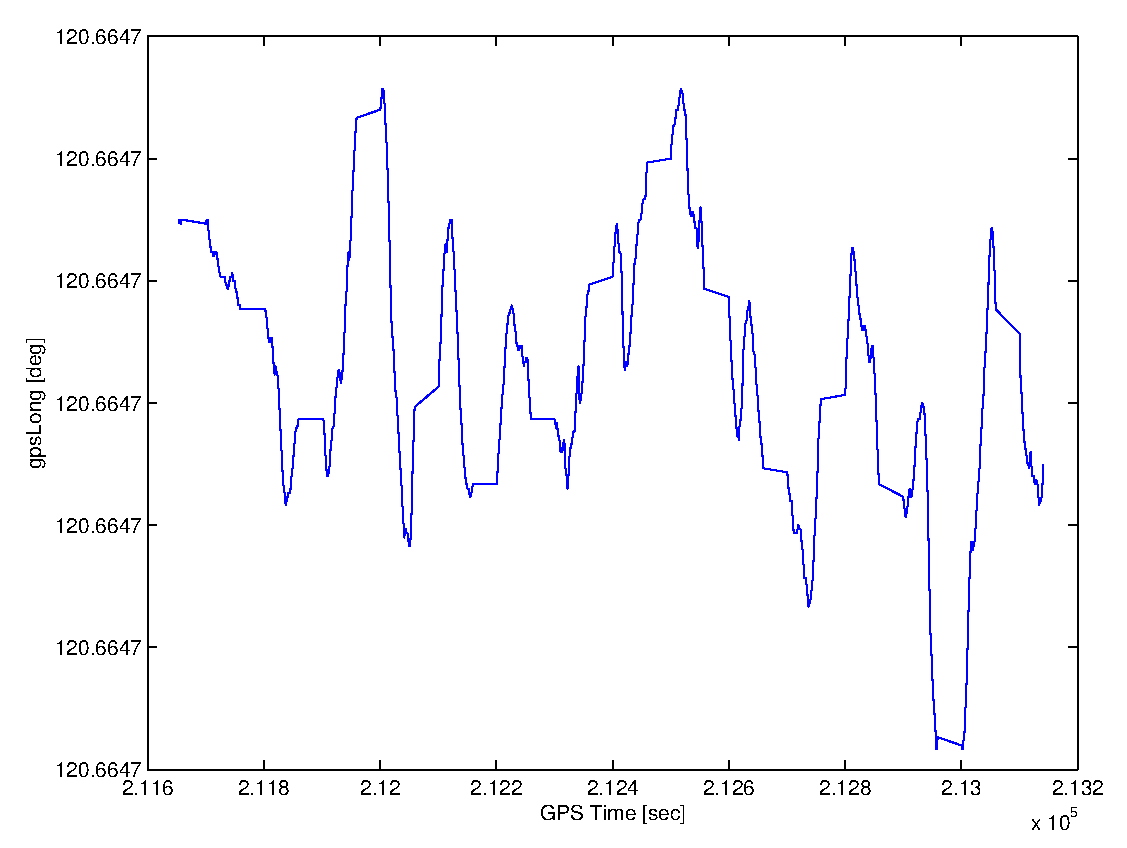
\includegraphics[width = 0.7\textwidth]{C:/Users/mufasa/Documents/Thesis/LaTex/figures/sampleOutput/Raw/gpsLong.eps}
\end{figure}
\begin{figure}[H]
	\centering
	\caption{gpsSpd vs. Time}
		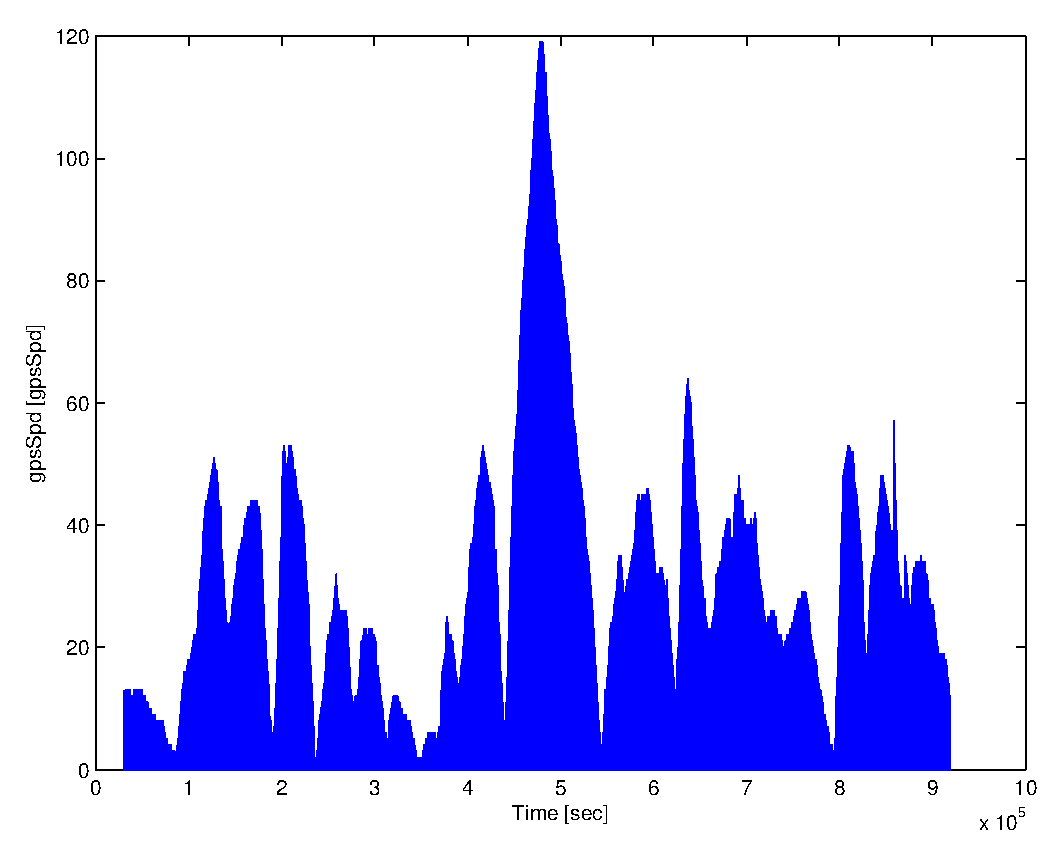
\includegraphics[width = 0.7\textwidth]{C:/Users/mufasa/Documents/Thesis/LaTex/figures/sampleOutput/Raw/gpsSpd.eps}
\end{figure}
\begin{figure}[H]
	\centering
	\caption{gpsCrs vs. Time}
		\includegraphics[width = 0.7\textwidth]{C:/Users/mufasa/Documents/Thesis/LaTex/figures/sampleOutput/Raw/gpsCrs.eps}
\end{figure}
\begin{figure}[H]
	\centering
	\caption{date vs. Time}
		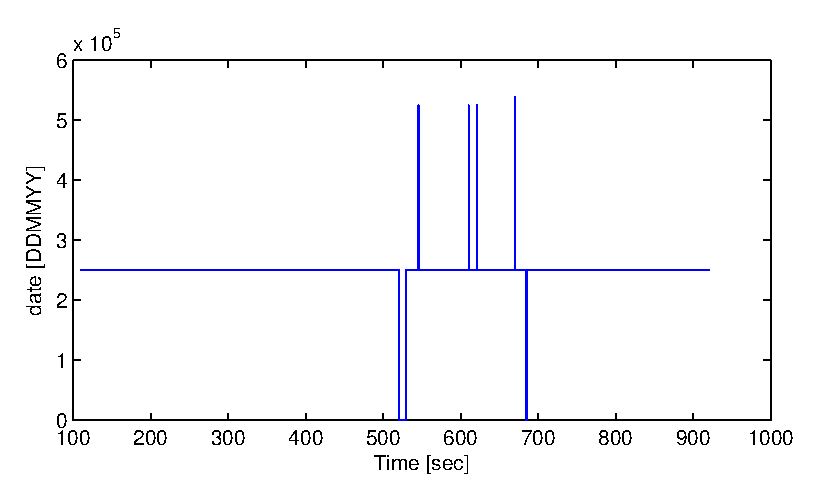
\includegraphics[width = 0.7\textwidth]{C:/Users/mufasa/Documents/Thesis/LaTex/figures/sampleOutput/Raw/date.eps}
\end{figure}
\begin{figure}[H]
	\centering
	\caption{CS vs. Time}
		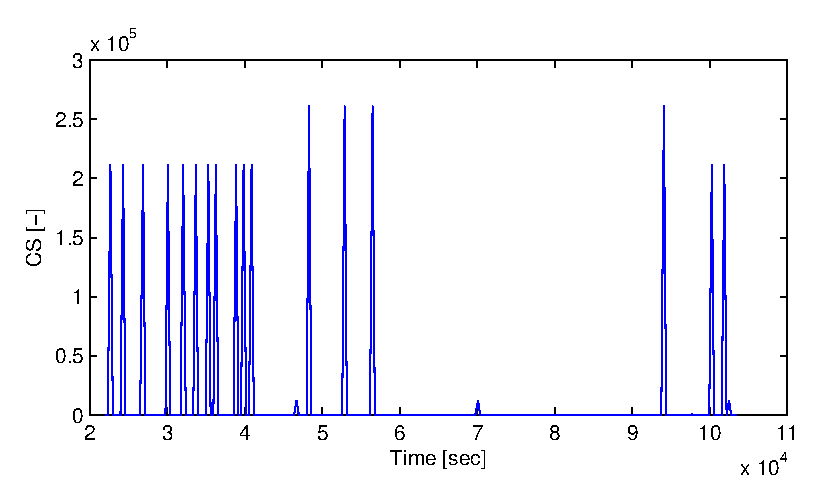
\includegraphics[width = 0.7\textwidth]{C:/Users/mufasa/Documents/Thesis/LaTex/figures/sampleOutput/Raw/CS.eps}
\end{figure}
\begin{figure}[H]
	\centering
	\caption{temperature vs. Time}
		\includegraphics[width = 0.7\textwidth]{C:/Users/mufasa/Documents/Thesis/LaTex/figures/sampleOutput/Raw/temperature.eps}
\end{figure}
\begin{figure}[H]
	\centering
	\caption{pwm0 vs. Time}
		\includegraphics[width = 0.7\textwidth]{C:/Users/mufasa/Documents/Thesis/LaTex/figures/sampleOutput/Raw/pwm0.eps}
\end{figure}
\begin{figure}[H]
	\centering
	\caption{pwm1 vs. Time}
		\includegraphics[width = 0.7\textwidth]{C:/Users/mufasa/Documents/Thesis/LaTex/figures/sampleOutput/Raw/pwm1.eps}
\end{figure}
\begin{figure}[H]
	\centering
	\caption{pwm2 vs. Time}
		\includegraphics[width = 0.7\textwidth]{C:/Users/mufasa/Documents/Thesis/LaTex/figures/sampleOutput/Raw/pwm2.eps}
\end{figure}
\begin{figure}[H]
	\centering
	\caption{pwm3 vs. Time}
		\includegraphics[width = 0.7\textwidth]{C:/Users/mufasa/Documents/Thesis/LaTex/figures/sampleOutput/Raw/pwm3.eps}
\end{figure}
\begin{figure}[H]
	\centering
	\caption{pwm4 vs. Time}
		\includegraphics[width = 0.7\textwidth]{C:/Users/mufasa/Documents/Thesis/LaTex/figures/sampleOutput/Raw/pwm4.eps}
\end{figure}
\begin{figure}[H]
	\centering
	\caption{pwm5 vs. Time}
		\includegraphics[width = 0.7\textwidth]{C:/Users/mufasa/Documents/Thesis/LaTex/figures/sampleOutput/Raw/pwm5.eps}
\end{figure}
\begin{figure}[H]
	\centering
	\caption{pwm6 vs. Time}
		\includegraphics[width = 0.7\textwidth]{C:/Users/mufasa/Documents/Thesis/LaTex/figures/sampleOutput/Raw/pwm6.eps}
\end{figure}
\begin{figure}[H]
	\centering
	\caption{pwm7 vs. Time}
		\includegraphics[width = 0.7\textwidth]{C:/Users/mufasa/Documents/Thesis/LaTex/figures/sampleOutput/Raw/pwm7.eps}
\end{figure}
\begin{figure}[H]
	\centering
	\caption{deltaT vs. Time}
		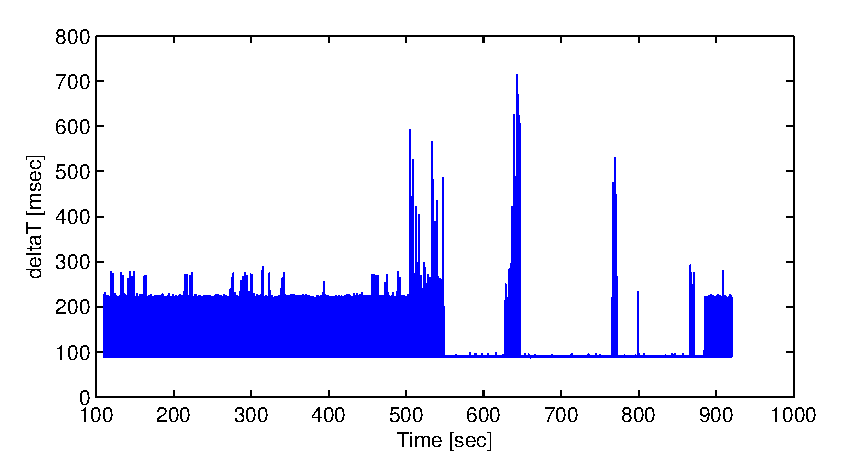
\includegraphics[width = 0.7\textwidth]{C:/Users/mufasa/Documents/Thesis/LaTex/figures/sampleOutput/Raw/deltaT.eps}
\end{figure}
